\documentclass{article}
\usepackage{tikz}
\usepackage{caption}
\title{Figure with Caption Fixture}
\author{Strata Reader Project}
\begin{document}
\maketitle

\section{Introduction}
This document contains a vector figure created using TikZ with an accompanying caption, designed to test the layout analysis and figure/caption association of Strata-Reader.

\section{Visual Representation}
Below is a diagram representing neural network layers.

\begin{figure}[h]
\centering
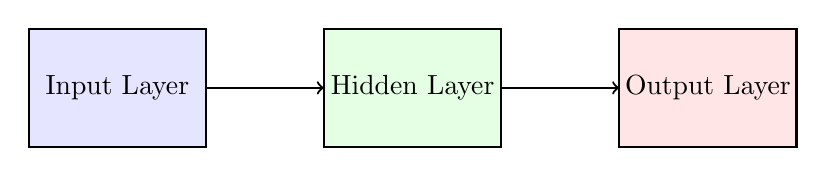
\begin{tikzpicture}[scale=1.5]
  \draw[thick, fill=blue!10] (0,0) rectangle (1.5,1) node[pos=.5] {Input Layer};
  \draw[thick, ->] (1.5,0.5) -- (2.5,0.5);
  \draw[thick, fill=green!10] (2.5,0) rectangle (4,1) node[pos=.5] {Hidden Layer};
  \draw[thick, ->] (4,0.5) -- (5,0.5);
  \draw[thick, fill=red!10] (5,0) rectangle (6.5,1) node[pos=.5] {Output Layer};
\end{tikzpicture}
\caption{A simple feedforward neural network structure with input, hidden, and output layers.}
\label{fig:nn}
\end{figure}

\end{document}
